\lecture{19}{May 15.}{}
\begin{definition}[Block]
    A block in a graph \(G\) is a maximal (under inclusion) induced connected subgraph with no cut-vertex, i.e. if the induced connected subgraph is \(H \subseteq G\), then remove any \(z \in V(H)\) will not disconnect \(H\).  
\end{definition}

\begin{corollary}
    A block is either an edge or 2-connected.
\end{corollary} 

\begin{lemma}
    Two blocks can share at most one vertex.
\end{lemma}
\begin{proof}
    If two blocks \(B_1, B_2\) share \(\ge 2\) vertices, then \(B_1 \cup B_2\) is connected without cut vertices, which contradicts to the maximality of \(B_1, B_2\).     
\end{proof}

\begin{remark}
    This lemma shows every edge is in a unique block. 
\end{remark}

\begin{figure}[H]
\centering
\begin{tikzpicture}[
    vertex/.style={circle, draw, fill=white, inner sep=1.5pt, minimum size=5pt},
    edge/.style={thick},
    blocklabel/.style={font=\small\bfseries}
]
    \node[vertex,label=above:\(a\)] (a) at (0,1.2) {};
    \node[vertex,label=left:\(b\)] (b) at (-1,0) {};
    \node[vertex,label=right:\(c\)] (c) at (1,0) {};
    \node[vertex,label=below:\(d\)] (d) at (0,-1.2) {};

    \node[vertex,label=above:\(e\)] (e) at (2.6,1.0) {};
    \node[vertex,label=below:\(f\)] (f) at (2.6,-1.0) {};
    \node[vertex,label=right:\(g\)] (g) at (4.0,0) {};

    \node[vertex,label=above:\(h\)] (h) at (5.7,1.0) {};
    \node[vertex,label=below:\(i\)] (i) at (5.7,-1.0) {};
    \node[vertex,label=right:\(j\)] (j) at (7.0,0) {};

    \node[vertex,label=above:\(k\)] (k) at (4.0,2.4) {};
    \node[vertex,label=above:\(\ell\)] (l) at (5.2,3.0) {};
    \node[vertex,label=right:\(m\)] (m) at (6.1,2.0) {};

    \node[vertex,label=below:\(n\)] (n) at (4.0,-2.4) {};
    \node[vertex,label=below:\(o\)] (o) at (5.2,-3.0) {};

    \draw[edge] (a)--(b)--(d)--(c)--(a) (b)--(c);
    \draw[edge] (c)--(e)--(g)--(f)--(c) (e)--(f);
    \draw[edge] (g)--(h)--(j)--(i)--(g) (h)--(i);
    \draw[edge] (g)--(k)--(l)--(m)--(g) (k)--(m);
    \draw[edge] (g)--(n)--(o)--(g);

    \begin{scope}[on background layer]
        \node[draw=blue!70, rounded corners, thick, fit=(a)(b)(c)(d), inner sep=11pt,
              label={[blue!70]above left:\(B_1\)}] {};
        \node[draw=red!70, rounded corners, thick, fit=(c)(e)(f)(g), inner sep=11pt,
              label={[red!70]above:\(B_2\)}] {};
        \node[draw=green!60!black, rounded corners, thick, fit=(g)(h)(i)(j), inner sep=11pt,
              label={[green!60!black]above:\(B_3\)}] {};
        \node[draw=orange!85!black, rounded corners, thick, fit=(g)(k)(l)(m), inner sep=11pt,
              label={[orange!85!black]above:\(B_4\)}] {};
        \node[draw=purple!75, rounded corners, thick, fit=(g)(n)(o), inner sep=11pt,
              label={[purple!75]below:\(B_5\)}] {};
    \end{scope}
\end{tikzpicture}
\caption{A connected graph decomposed into five blocks.  Consecutive blocks meet only at cut-vertices such as \(c\) and \(g\), and every vertex belongs to at least one block.}
\end{figure}

\begin{proposition}
    Let \(G\) be a connected graph.  Define the block/cut-vertex graph \(\Gamma\) as follows: the vertices of \(\Gamma\) are the blocks of \(G\) together with the cut-vertices of \(G\), and a block \(B\) is adjacent to a cut-vertex \(v\) precisely when \(v \in V(B)\).  Then \(\Gamma\) is a tree.
\end{proposition}

\begin{proof}
    We prove that \(\Gamma\) is connected and acyclic.

    First, \(\Gamma\) is connected.  Let \(X\) and \(Y\) be two vertices of \(\Gamma\).  If \(X\) is a block, choose a vertex \(x \in V(X)\); if \(X\) is a cut-vertex, let \(x=X\).  Choose \(y\) from \(Y\) in the same way.  Since \(G\) is connected, there is an \(x\)-to-\(y\) path in \(G\).  Each edge of this path lies in a unique block.  As we move along the path, whenever we pass from one block to another, the two blocks meet in a common vertex.  Such a common vertex must be a cut-vertex; otherwise the two blocks could be joined to form a larger connected subgraph with no cut-vertex, contradicting maximality of blocks.  Therefore the path in \(G\) gives a walk in \(\Gamma\) from \(X\) to \(Y\).  Hence \(\Gamma\) is connected.

    \begin{figure}[H]
    \centering
    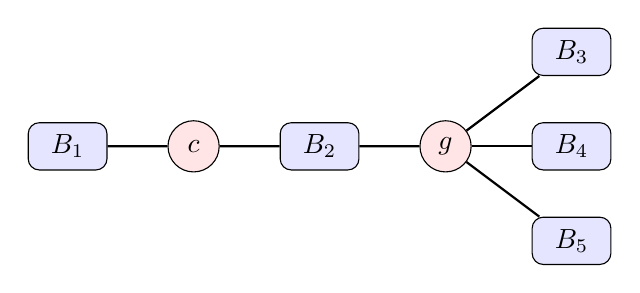
\begin{tikzpicture}[
        block/.style={rectangle, draw, rounded corners, fill=blue!10, minimum width=1cm, minimum height=.6cm},
        cut/.style={circle, draw, fill=red!10, minimum size=.65cm},
        treeedge/.style={thick}
    ]
        \node[block] (B1) at (0,0) {\(B_1\)};
        \node[cut] (c) at (1.6,0) {\(c\)};
        \node[block] (B2) at (3.2,0) {\(B_2\)};
        \node[cut] (g) at (4.8,0) {\(g\)};
        \node[block] (B3) at (6.4,1.2) {\(B_3\)};
        \node[block] (B4) at (6.4,0) {\(B_4\)};
        \node[block] (B5) at (6.4,-1.2) {\(B_5\)};

        \draw[treeedge] (B1)--(c)--(B2)--(g)--(B3);
        \draw[treeedge] (g)--(B4);
        \draw[treeedge] (g)--(B5);
    \end{tikzpicture}
    \caption{The block/cut-vertex graph \(\Gamma\) for the preceding example.  Rectangles represent blocks and circles represent cut-vertices.}
    \end{figure}

    It remains to show that \(\Gamma\) has no cycle.  Suppose, for a contradiction, that \(\Gamma\) contains a cycle
    \[
        B_1, v_1, B_2, v_2, \ldots, B_k, v_k, B_1,
    \]
    where each \(B_i\) is a block and each \(v_i\) is a cut-vertex.  Let
    \[
        H = B_1 \cup B_2 \cup \cdots \cup B_k.
    \]
    The subgraph \(H\) is connected, because consecutive blocks in the cycle meet at the vertices \(v_i\).  Moreover, no vertex of \(H\) is a cut-vertex of \(H\).  Indeed, removing a vertex from one block cannot disconnect that block, and the cyclic arrangement gives another route through the remaining blocks whenever one of the shared vertices \(v_i\) is removed.  Thus \(H\) is a connected subgraph with no cut-vertex that properly contains each \(B_i\), contradicting the maximality of the blocks.  Hence \(\Gamma\) is acyclic.

    Since \(\Gamma\) is both connected and acyclic, \(\Gamma\) is a tree.
\end{proof}

\begin{corollary}
    \(\Gamma \) has leaves iff blocks in \(G\).  
\end{corollary}

\begin{proof}
    By the proposition, \(\Gamma\) is a tree.

    We claim that no cut-vertex of \(G\) can be a leaf of \(\Gamma\).  Indeed, if \(v\) is a cut-vertex of \(G\), then \(G-v\) has at least two connected components.  Since \(G\) is connected, each such component contains a neighbor of \(v\).  The edge from \(v\) to such a neighbor lies in some block containing \(v\).  Edges going from \(v\) into two different components of \(G-v\) cannot lie in the same block; otherwise that block would contain a path between the two components after removing \(v\), contradicting that they are different components of \(G-v\).  Hence \(v\) belongs to at least two distinct blocks.

    Therefore the vertex \(v\) of \(\Gamma\) is adjacent to at least two block-vertices, so its degree in \(\Gamma\) is at least two.  Thus a leaf of \(\Gamma\) cannot be a cut-vertex; every leaf of \(\Gamma\) must be a block-vertex.
\end{proof}

Now we can give the proof of Brook's theorem: If \(G\) is not complete or an odd cycle, then 
\[
    \chi (G) \le \Delta (G).
\] 

\begin{proof}[proof of Brook's theorem]
    Idea: find a rooted spanning tree of $G$. Run the greedy coloring algorithm, processing vertices from the leaves up to the root.

    Then, in this coloring, every non-root vertex $v$ is colored before its ancestor, and so at most $d(v)-1 \le \Delta(G)-1$ colors unavailable (its parent has not been colored when we color a non-root vertex). Therefore, we may color it with one of the first $\Delta(G)$ vertices. Now the goal is to choose a good root vertex to color in the last so that we can color \(G\) legally. 

    {\bf Case 1.} $G$ has a vertex $v$ with $d(v)<\Delta(G)$.

    Then we make $v$ the root. Then $v$ will have $<\Delta(G)$ unavailable colors, and so we can color it with $[\Delta(G)]$.

    {\bf Case 2.} $G$ has a cut-vertex $v$.

    We make $v$ the root and $\Delta$-color $G-v$. Then if $v$ has no color available, we may permute the colors on one of the components of $G-v$ to free up a color for $v$.

    \begin{remark}
        Since \(v\) is a cut-vertex, so \(G - v\) is disconnected and thus has two distinct components \(C_1, C_2\). Now if we regard \(v\) as the root of the spanning tree, and run the coloring algorithm above, and when we color \(v\), no colors are left, then \(v\) has \(\Delta (G)\) neighbors, and all neighbors of \(v\) uses different colors. Now suppose the set of vertices of \(C_i\) adjacent to \(v\) is \(N_i\), then \(N_1 \cup N_2\) contains all \(\Delta (G)\) colors, and if color \(c\) is used by some vertex of \(N_2\), and \(c^{\prime} \) is some color used by vertex of \(N_1\), we can interchange the colors of vertices in \(C_1\) using \(c\) and \(c^{\prime}\). Note that this would not make the coloring improper since \(C_1\) and \(C_2\) are disconnect, and interchange colors in a properly colored component will not break the coloring. Thus, we can color \(v\) by \(c^{\prime}\) after interchanging colors.                     
    \end{remark}

    The left cases are \(d(v) = \Delta (G)\) for all \(v \in V(G)\) and \(G\) has no cut-vertices:   

    {\bf Case 3.} $G$ is $k$-regular without cut-vertices.

    {\bf Case 3-1.} $k \le 2$ or $k=|V(G)|-1$.

    This implies that $G$ is either a cycle (\(k = 2\)) or \(K_n\).

    {\bf Case 3-2.} $G$ is $k$-regular ($3 \le k \le n-2$) and 2-connected (has no cut-vertcies).

    Want: a vertex $v_n$ with two non-adjacent neighbors $v_1,v_2$ such that $G\setminus\{v_1,v_2\}$ is connected.

    If we have such \(v_1, v_2\), we can find a spanning tree of \(G \setminus \left\{ v_1, v_2 \right\} \), and adding \(\left\{ v_n, v_1 \right\} \) and \(\left\{ v_n, v_2 \right\} \) to attain a spanning tree of \(G\), which allows us to permutate colors as Case 2 since \(\left\{ v_1 \right\}, \left\{ v_2 \right\}  \) are two disconnected components in \(G \setminus \left\{ v_1, v_2 \right\} \).      

    Let $x$ be an arbitrary vertex.

    {\bf Case 3-2-1.} $\kappa(G-x) \ge 2$.

    Let $x=v_1$, and let $v_2$ be a vertex at distance 2 from $x$ (so \(x, v_2\) are not adjacent) and let $v_n$ be a common neighbor of $v_1$ and $v_2$.

    \begin{remark}
        Such \(v_2, v_n\) can be found since \(k \le n - 2\), so \(\exists w \in V(G)\) s.t. \(w \notin N(x)\). Hence, we can consider the shortest path from \(x\) to \(w\) on \(G\), say \(P\). Then, consider the first vertex of \(P\) that is not a neighbor of \(x\) or \(x\). Then, this vertex is at distance 2 from \(x\), and we can pick it as \(v_2\) and its previous vertex on \(P\) as \(v_n\).             
    \end{remark}

    {\bf Case 3-2-2.} $\kappa(G-x) =1$.

    Consider the leaf blocks of $G-x$. $x$ must have a neighbor in each leaf block (that is not a cut-vertex). Let $x=v_n$, $v_1,v_2$ be neighbors from different leaf blocks.

    \begin{remark}
        Since \(\kappa (G - x) = 1\), there is cut-vertex of \(G - x\), so \(G - x\) has at least two blocks. If \(C\) is a leaf block of \(G - x\), we can show \(x\) is adjacent to some vertex of \(C\) which is not cut-vertex. If not, say \(C\) contains a cut vertex \(w\), then \(x\) is adjacent to only \(G - (C - w)\). However, now if we remove \(w\) from \(G\), \(G - w\) is disconnected, which contradicts to the \(2\)-connectivity of \(G\).              
    \end{remark}
\end{proof}